\documentclass[]{scrartcl}
\usepackage{graphicx}
\usepackage{float}
\usepackage[breaklinks=true]{hyperref}
\usepackage{url}
\usepackage{listings}

%opening
\title{CRIMSON Build instructions for Windows}
\author{Marija Marcan}

\begin{document}

\maketitle

\begin{abstract}

\end{abstract}

\section{Dependencies to install before building CRIMSON}
Before building CRIMSON software itself you will need to download and install the following:

\begin{itemize}
	\item Git - 2.19.2 or later (\url{https://git-scm.com/downloads})
	\item CMake - 3.13.0 (\url{https://cmake.org/download/})
	\item Qt - 5.7 (exactly) - best to install using Qt's Unified Windows Installer. From all the components under 5.7 you only need "msvc2013 64-bit", "Qt WebEngine" and "Qt Script"
	\item Visual Studio - VS2013 
\end{itemize}



For installing the above software follow the instructions as provided by their publisher.
\linebreak
\\
Please note that the CRIMSON build procedure has been tested and is supported for the versions of software mentioned above. While it might be possible to succesfully build CRIMSON using other versions of Git, CMake or Visual Studio it is not necessary that the CRIMSON build steps as described below would be sufficient, so proceed at your own responsibility.

\section{Building CRIMSON}
\subsection{Setup the project directory}
Create a root folder in which the source code and build will be stored.
The root folder for the project should be as short as possible (due to some limitations of the Windows command line). 
For example, a source folder like "\path{C:\CRIMSON}" and a build folder like "\path{C:\CRIMSON\sb}" should be good enough.
\subsection{Get the source code via Git}
Get the source code via git by cloning into the root folder selected above by following these steps:

\begin{enumerate}
	\item Open the Windows Command Prompt (Windows - type "cmd" - press Enter).
	\item Change the current working directory to the location of project root directory. e.g. for root directory "\path{C:\CRIMSON}" type 
	\begin{lstlisting}
	cd c/CRIMSON
	\end{lstlisting} 
	into the command prompt and press Enter.
	\item Type 
	\begin{lstlisting}
	git clone https://username@bitbucket.org/cafa/crimson.git .
	\end{lstlisting}
	(Notice the dot at the end of the above command, it is there intentionally!)
	\\and press "Enter". 
	\item Enter your bitbucket password when prompted.
\end{enumerate}

\subsection{Generate project files with CMake}
\begin{enumerate}
	\item In the root folder of the CRIMSON project create a new folder for the build, e.g. "\path{C:\CRIMSON\sb}"
	\item Open the CMake desktop app.
	\item Under "Where is the source code" enter the path to the CRIMSON root folder (e.g. "\path{C:\CRIMSON}")
	\item Under "Where to build the binaries" enter the path to the CRIMSON build folder you created just recently (e.g. "\path{C:\CRIMSON\sb}")
	
	\begin{figure}[H]
		\centering
		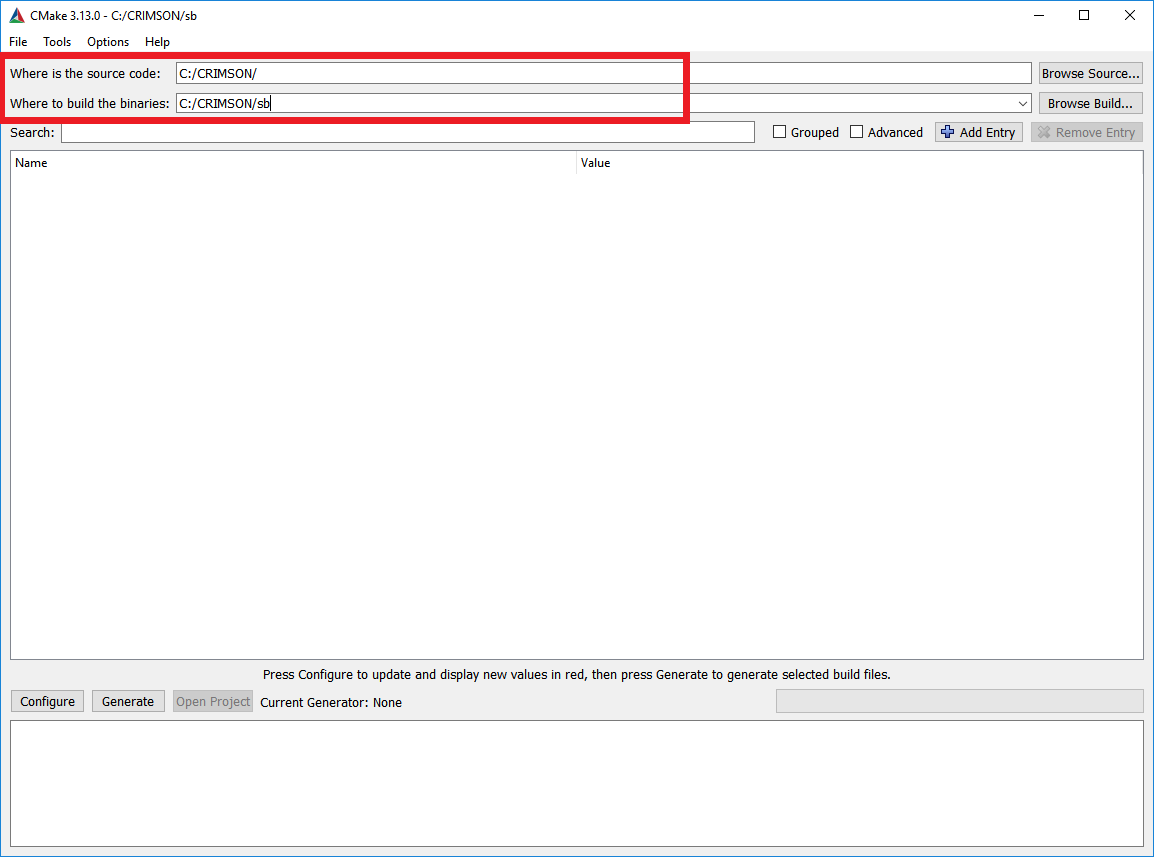
\includegraphics[width=0.8\linewidth]{Images/folders}
		\caption{Specifying source and build directories}
		\label{fig:folders}
	\end{figure}

	\item Press "Configure"
	\item In the new window that pops up, under "Specify the generator for this project" select "Visual Studio 12 2013 Win64". Leave the remaining settings as they are and press "Finish".
	
	\begin{figure}[H]
		\centering
		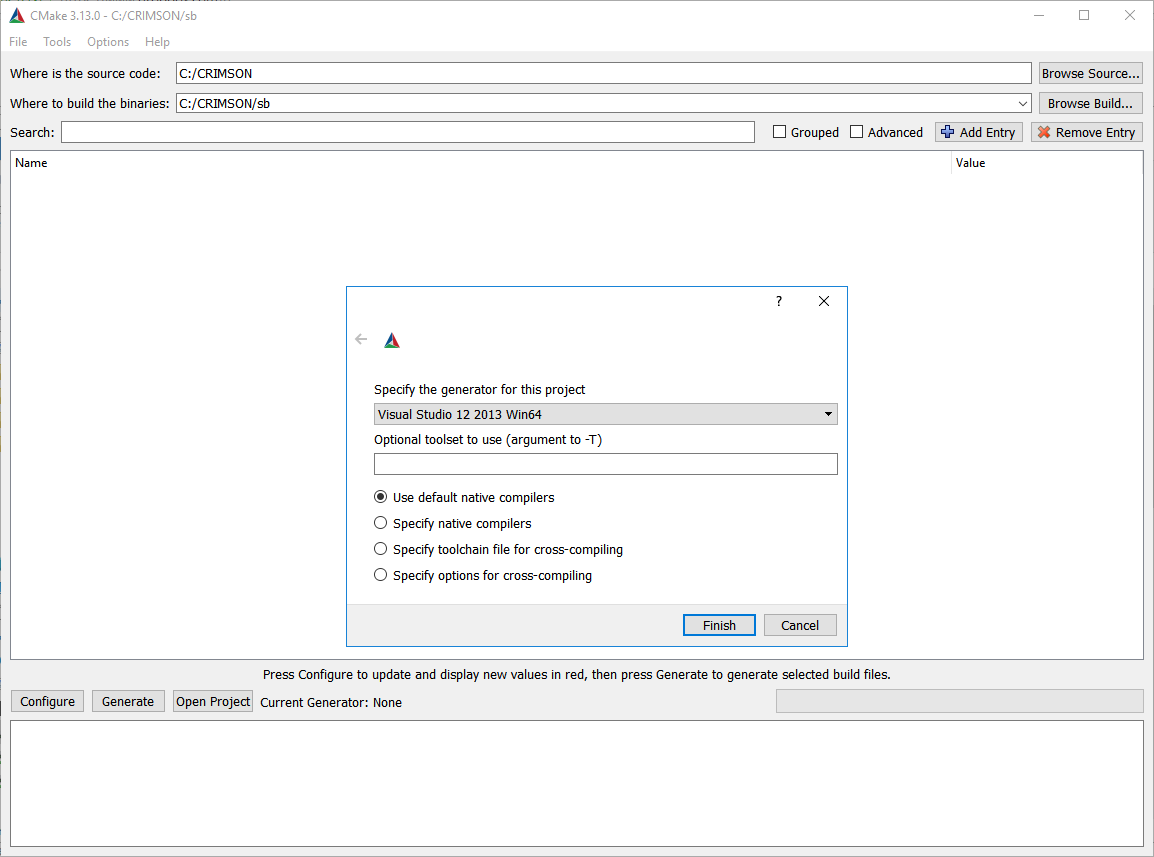
\includegraphics[width=0.8\linewidth]{Images/cmake2}
		\caption{Specify project generator}
		\label{fig:cmake2}
	\end{figure}
	
	\item An error message pops up. Press okay to continue.
	
	\begin{figure}[H]
		\centering
		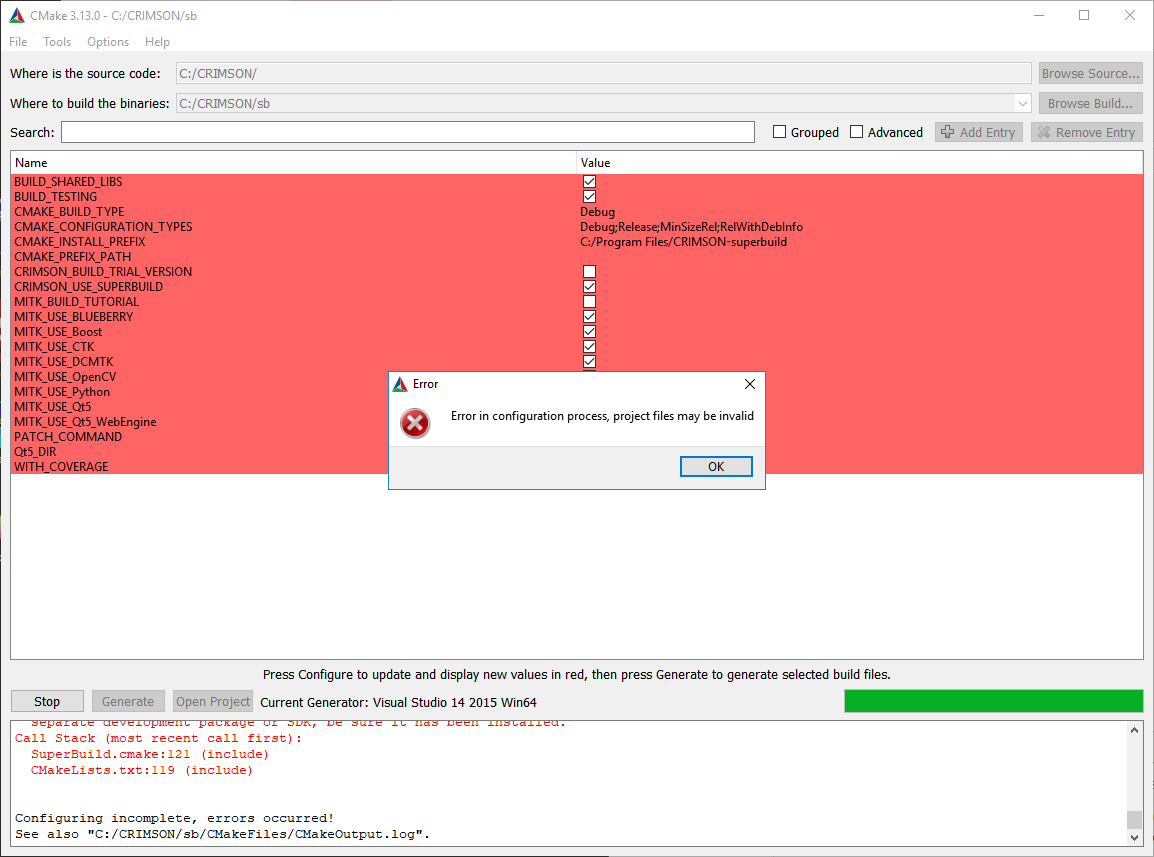
\includegraphics[width=0.8\linewidth]{Images/cmake3}
		\caption{An expected error}
		\label{fig:cmake3}
	\end{figure}
	\item The large window in the centre now contains pairs of variable names and values colored red, some of which need to be manually set for a succesfull build. Find a variable "Qt5\_DIR" and set it to "\path{C:\Qt\5.7\msvc2013_64\lib\cmake\Qt5}" (assuming that you installed Qt in the default directory "\path{C:\Qt}", otherwise replace the "Qt" part by the path which you chose during Qt installation).
	\item Change CMAKE\_BUILD\_TYPE as desired (Release, Debug or RelWithDebInfo). Leave other variables as they are.
	\item Press "Configure".
	\item Additional variables that can be modified appear now. You need to manually specify the locations of flowsolver and presolver:
	\begin{itemize}
		\item For "flowsolver\_folder" enter e.g. "\path{C:\CRIMSON\sb\CMakeExternals\Source\flowsolver}"
		\linebreak Note: This is simply a stub folder for where CRIMSON expects flowsolver files to be located. Actual flowsolver files are copied there after running the separate flowsolver installer.
		\item For "presolver\_executable" enter e.g. "\path{C:\CRIMSON\sb\CMakeExternals\Source\presolver\presolver.exe}".
		In variables above replace "\path{C:\CRIMSON\sb}" with your own custom location of CRIMSON superbuild folder as necessary.
	\end{itemize}

	\item Press "Configure"
	\item Press "Generate"
	
\end{enumerate}

\subsection{Build your project in Visual Studio}

\begin{enumerate}
	\item Open the build folder of the project which you have previously created (in our example this is "\path{C:\CRIMSON\sb}").
	The folder contains project files which were generated by CMake for our selected version of Visual Studio (2013). These Visual Studio files belong to the CRIMSON superbuild (build configuration which automatically builds CRIMSON with all of its external dependencies, one of which is MITK. Note here that the MITK itself also has its own external dependencies). 
	\\Inside the overall superbuild CRIMSON project, MITK and its dependencies are being built in a superbuild project of their own (inside the folder "MITK-superbuild"). Project files for building of other external dependencies of CRIMSON are located in folder "CMakeExternals". The project files for building of CRIMSON core are in folder "CRIMSON-build".
	\item In the CRIMSON superbuild folder ("\path{C:\CRIMSON\sb}") open the file named "CRIMSON-superbuild" of the type "Microsoft Visual Studio Solution". This opens the CRIMSON superbuild project in Visual Studio.
	\item Make sure that the build type selected in Visual Studio matches the build type you determined in CMake (sometimes these types do not automatically match).
	
	\begin{figure}[H]
		\centering
		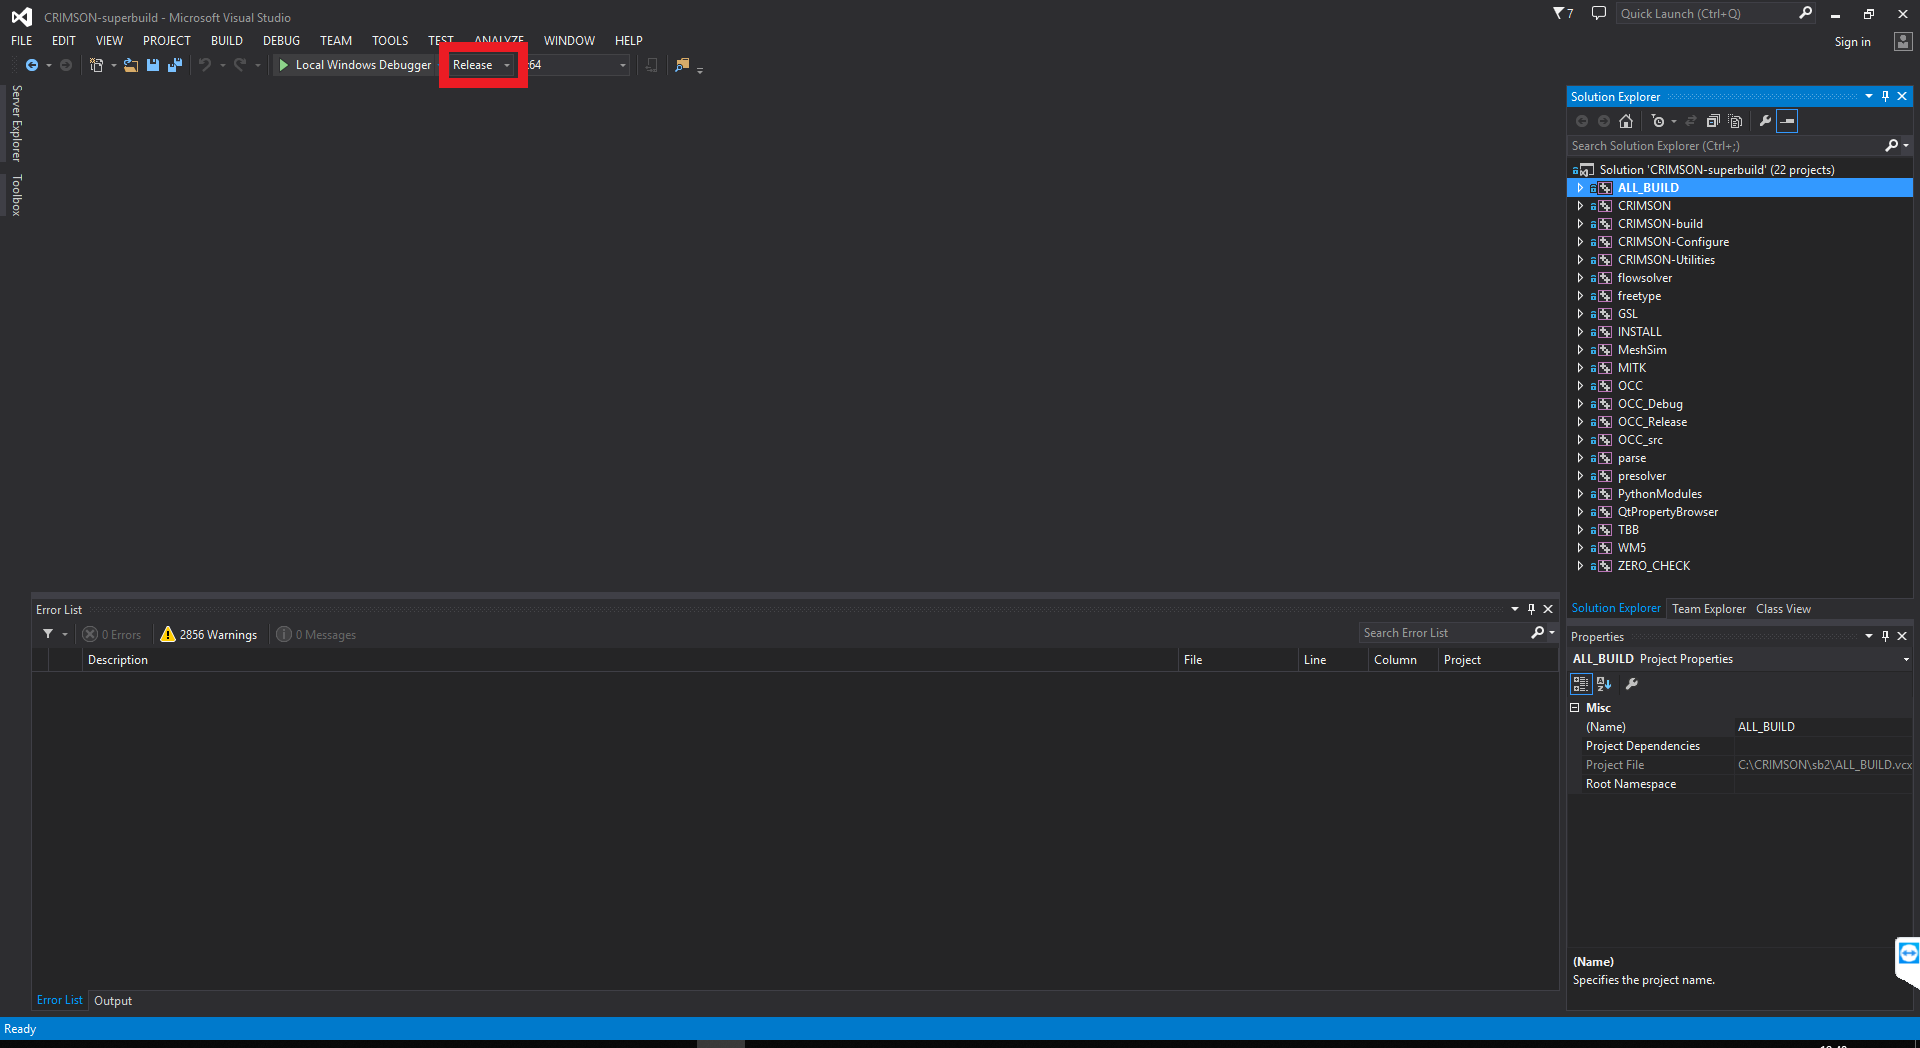
\includegraphics[width=0.9\linewidth]{Images/vs}
		\caption{Build type}
		\label{fig:vs}
	\end{figure}
	\item In order to avoid known collision between an "fttypes.h" header that exists under project "freetype" and in standard Windows Kit 8.1 (same name, different contents), do the following:
	\begin{enumerate}
		\item In the Solution Explorer pane on the right, right-click the node "freetype" and select "Properties" (last entry). 
		\item On the left side of the new window that pops up select "VC++ Directories"
		\item Click on "Include Directories" on the right side, and then on the down arrow on the very end of that line to edit the field.
		\item In the drop-down menu select "Edit..."
		
		\begin{figure}[H]
			\centering
			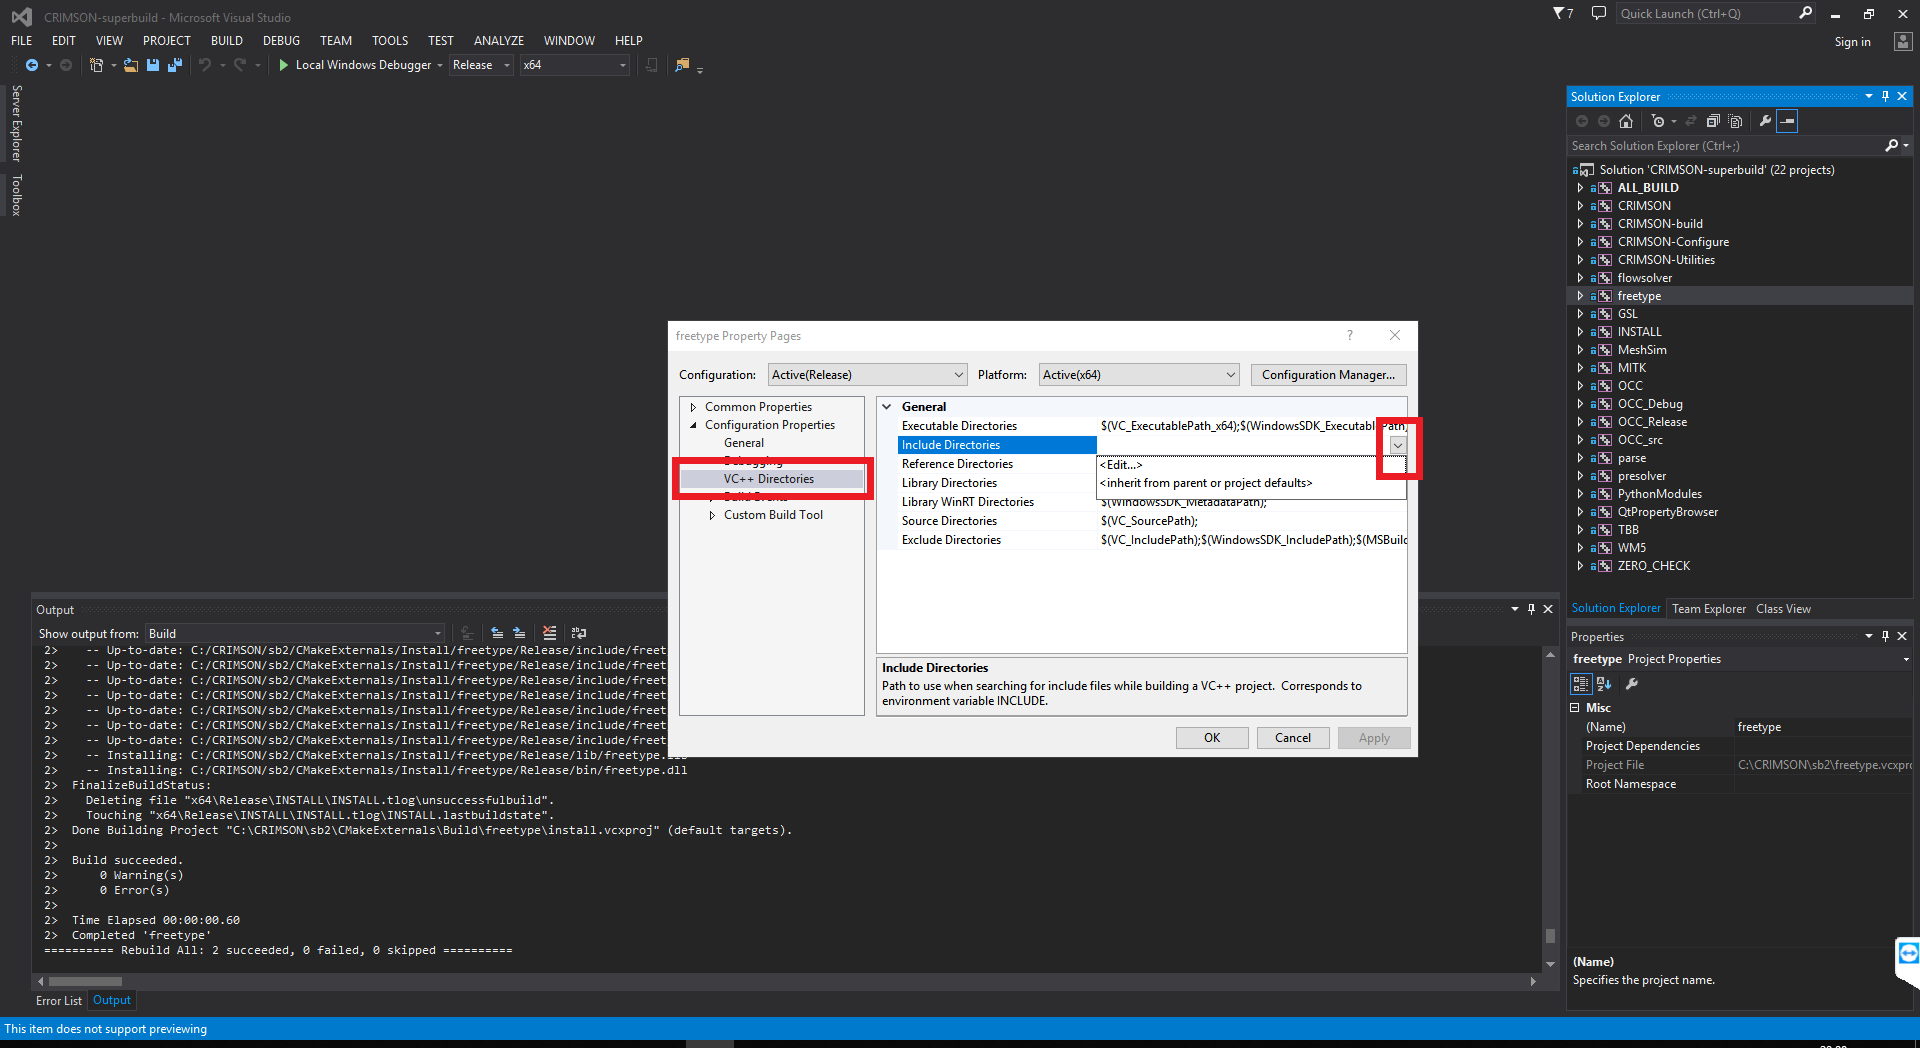
\includegraphics[width=0.9\linewidth]{Images/vs4}
			\caption{Project modification}
			\label{fig:vs4}
		\end{figure}
	
		\item On the bottom of the new window, make sure the field "Inherit from parent or project defaults" is UNTICKED
		
		\begin{figure}[H]
			\centering
			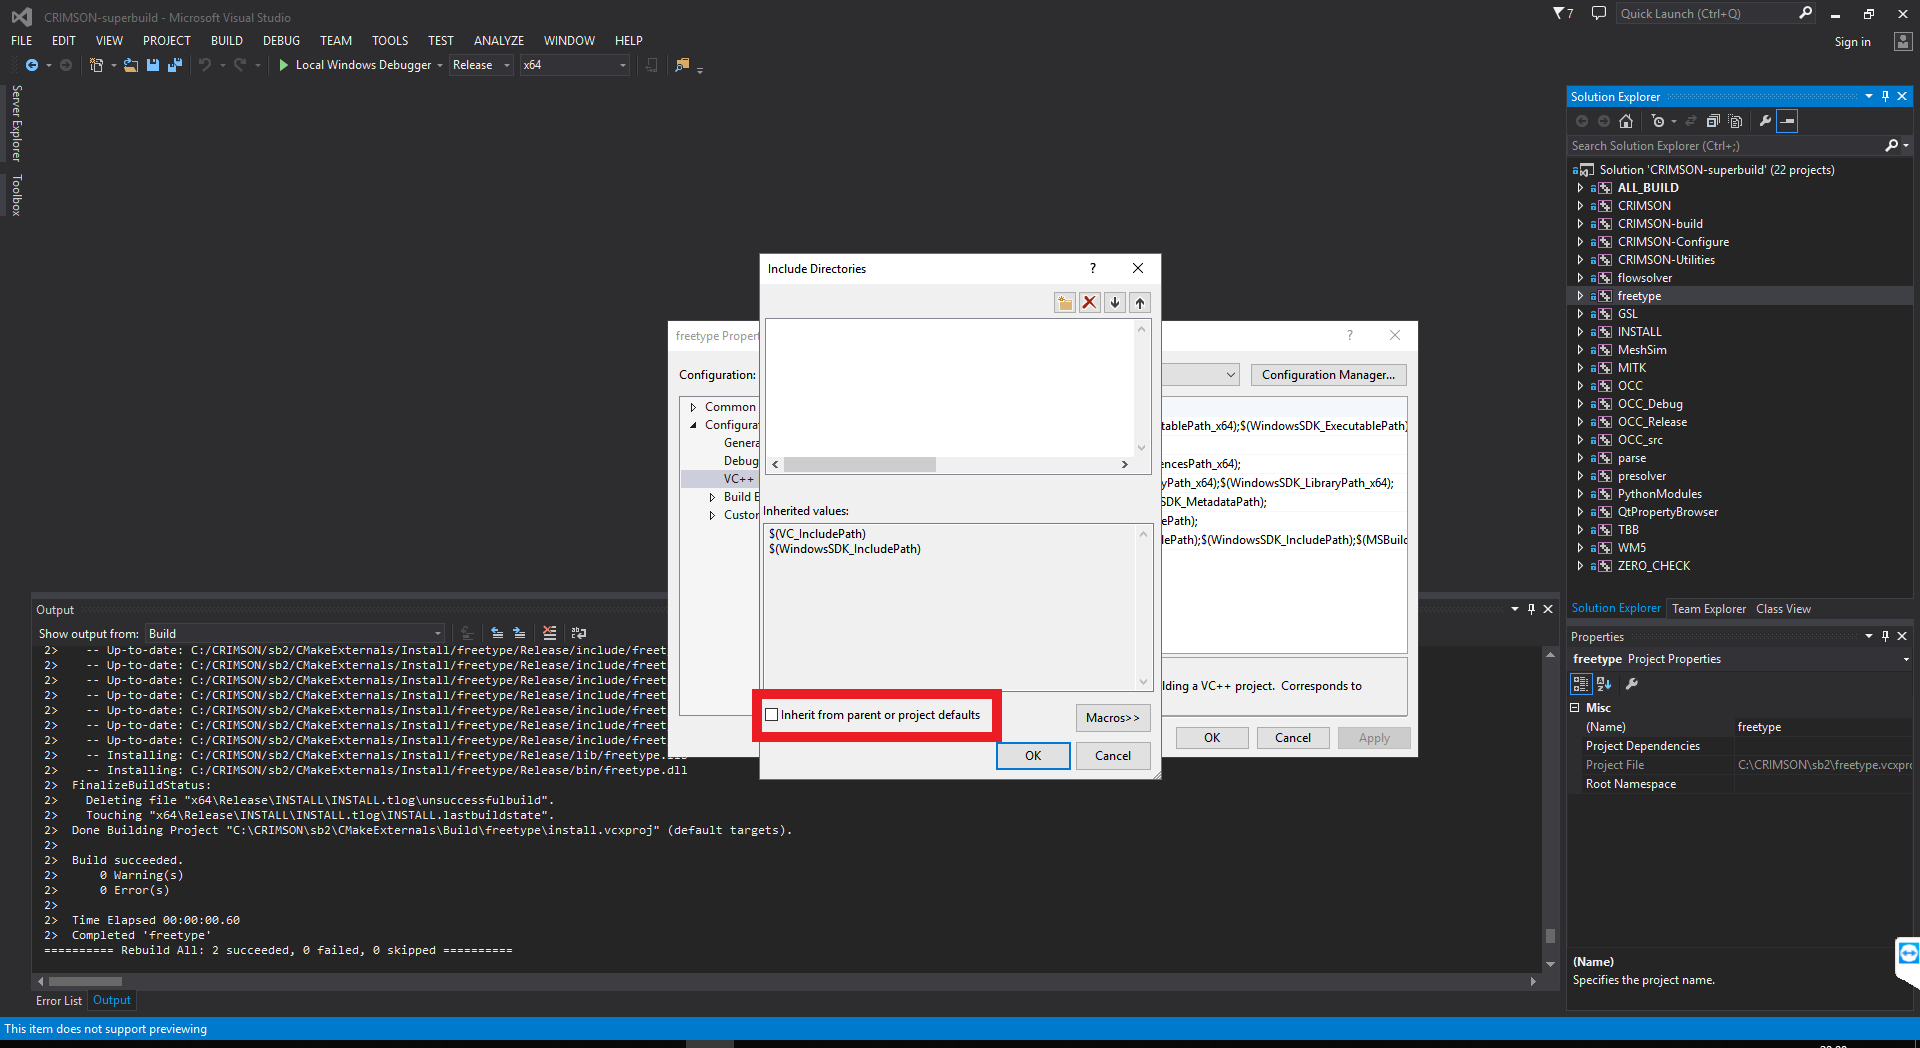
\includegraphics[width=0.9\linewidth]{Images/vs5}
			\caption{Project modification}
			\label{fig:vs5}
		\end{figure}
	
	\end{enumerate}

	\item In the Solution Explorer pane on the right, right-click the "ALL\_BUILD" node and press "Build"
	
	\begin{figure}[H]
		\centering
		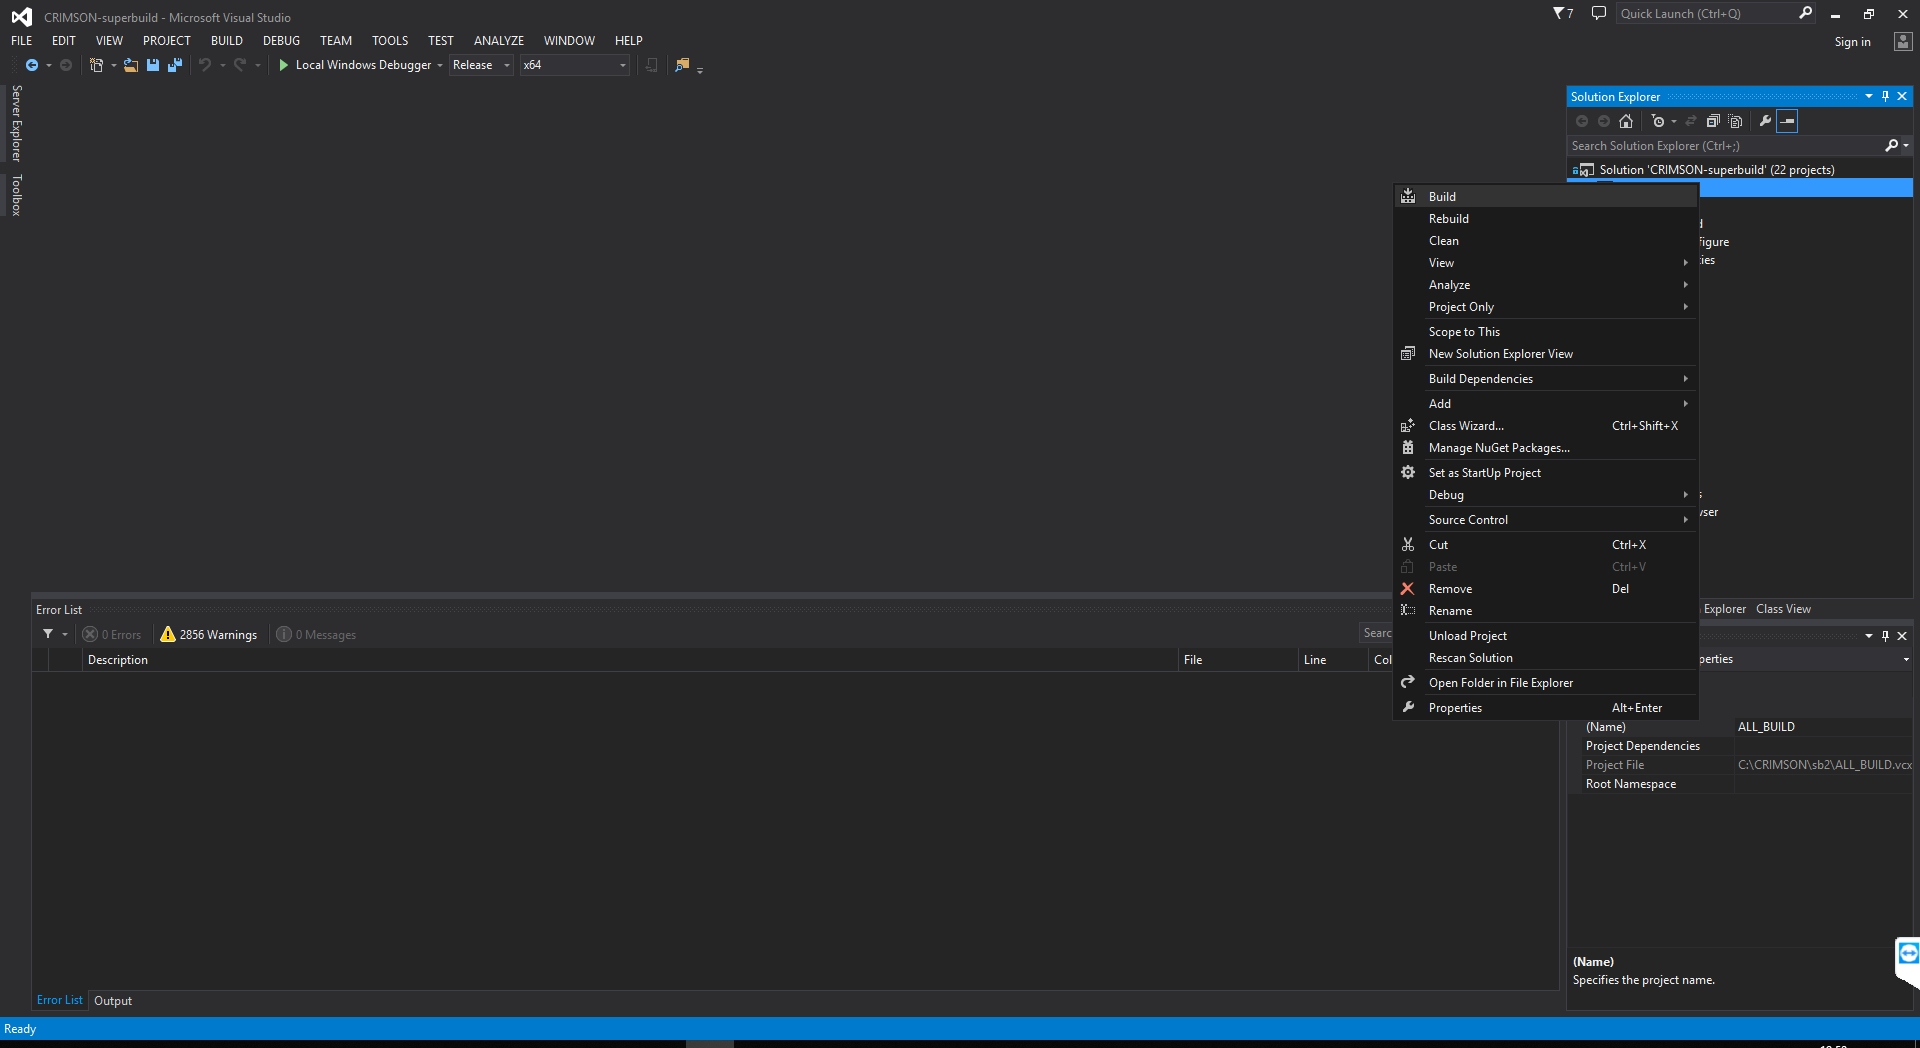
\includegraphics[width=0.9\linewidth]{Images/vs2}
		\caption{Building}
		\label{fig:vs2}
	\end{figure}
	\item Wait for all the project files to build. You can observe the progress in the "Output" window.
 
\end{enumerate}

\section{Running the built project inside Visual Studio}
\begin{itemize}
	\item In order to run CRIMSON from Visual Studio (e.g. for debugging purposes) navigate to the CRIMSON build folder ("\path{C:\CRIMSON\sb\CRIMSON-build}") and open the file named "CRIMSON" of the type "Microsoft Visual Studio Solution". This opens the CRIMSON core build project in Visual Studio.
	\item Right-click on the node "CRIMSON" in Solution Explorer and select "Set as StartUp project"
	
	\begin{figure}[H]
		\centering
		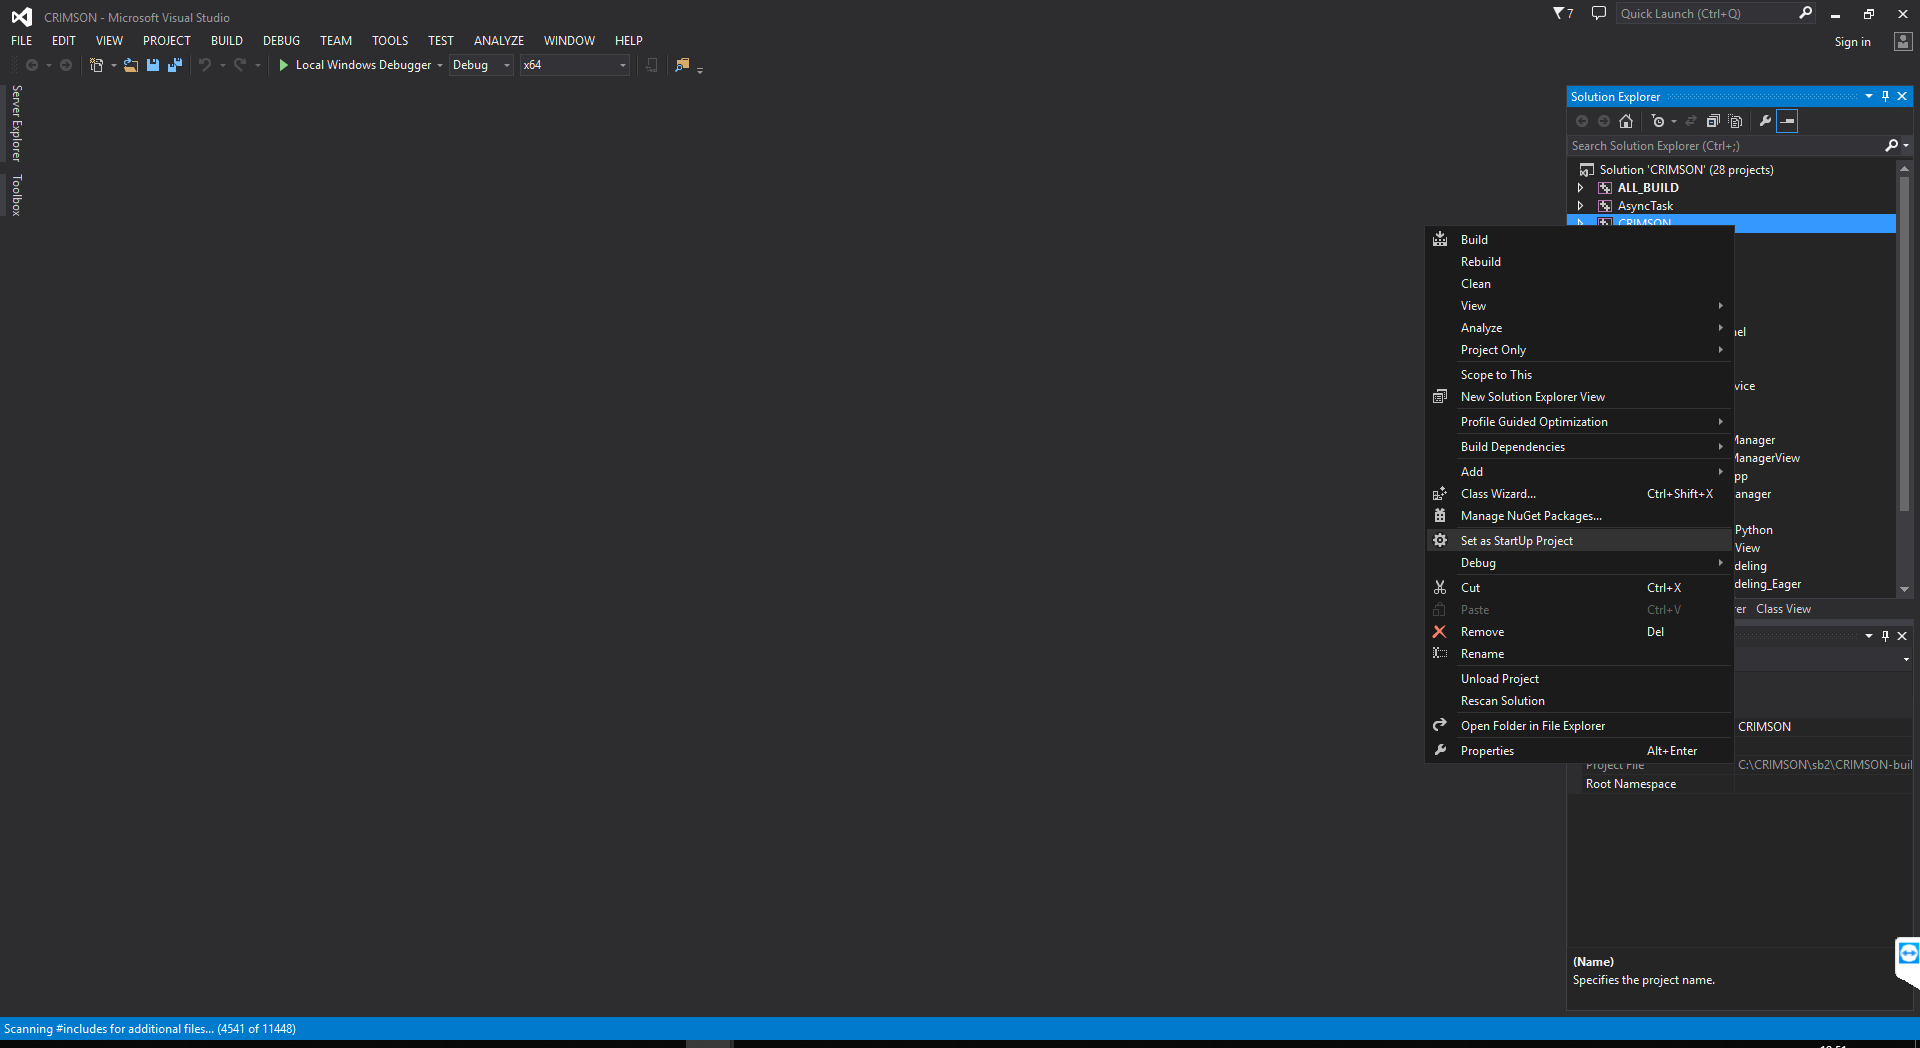
\includegraphics[width=0.9\linewidth]{Images/vs3}
		\caption{Set up for running}
		\label{fig:vs3}
	\end{figure}
	
	\item You are now ready to run/debug CRIMSON from within Visual Studio.
\end{itemize}

\section{Building CRIMSON install files (packaging)}

\begin{itemize}
	\item Open the CRIMSON core project from the CRIMSON-build folder (step 1. from the previous paragraph).
	\item In Solution Explorer right-click the node "PACKAGE" and select "Build".
	\item Wait for the project to be packaged and install files generated. You can observe the progress in the "Output" window.
	\item Once the packaging has succesfully finished the install file can be found in the CRIMSON-build folder.
\end{itemize}

\section{Adding flowsolver to your CRIMSON build}

\begin{itemize}
	\item Run the flowsolver installer. 
	\item Make sure to specify the same folder for unpacking as the one specified under "flowsolver\_folder" variable during CMake configuration.
\end{itemize}

\end{document}
